%%%%%%%%%%%%%%%%%%%%%%%%%%%%%%%%%%%%%%%%
%%%%%  xPhO LaTeX Beamer Template  %%%%%
%%%%%  Date: 17/03/2025            %%%%%
%%%%%  Authors:                    %%%%%
%%%%%       Nguyen Thanh Long      %%%%%
%%%%%       Nguyen Le Mai Huong    %%%%%
%%%%%       Nguyen Minh Phuong     %%%%%
%%%%%%%%%%%%%%%%%%%%%%%%%%%%%%%%%%%%%%%%

\documentclass[aspectratio=169, t]{beamer} % Ratio 16:9
\usepackage[T5]{fontenc}
\usepackage{lmodern}
\usepackage{graphicx} 
\usepackage{array}
\usepackage{longtable} % for long table

\usepackage{amsmath}

\usepackage{chngcntr}
\counterwithin{figure}{section}

\renewcommand{\familydefault}{\sfdefault} % Font

\usepackage{caption}
\usepackage{siunitx}

% \definecolor{BlueDefault}{rgb}{0.2,0.2,0.7}
\definecolor{BlueDefault}{RGB}{14,47,95}


% Hide navigation 
\setbeamertemplate{navigation symbols}{}

% Setup background
\newcommand{\normalbackground}{%
    \usebackgroundtemplate{
\includegraphics[width=\paperwidth,height=\paperheight]{Background/Normal_slide_xPhO.pdf}}%
}

\newcommand{\titlebackground}{%
    \usebackgroundtemplate{
\includegraphics[width=\paperwidth,height=\paperheight]{Background/Title_slide_xPhO.pdf}}%
}

% Change the title color to white
\setbeamercolor{frametitle}{fg=white} 

% push the title up by \raisebox
\setbeamertemplate{frametitle}{%
    \vspace{0.3em}
    \hspace{-1em} \insertframetitle
    % \vspace{2mm}
}

% Number of slide
\setbeamertemplate{footline}{%
    \hfill
    \insertframenumber/\inserttotalframenumber
    \hspace{7.5mm}
    \vspace{3.5mm}
}

%% Make Table of Contents %%
\AtBeginSection[]{
  \begin{frame}
  \frametitle{Mục lục}
  \tableofcontents[currentsection]
  \end{frame}
}

%% Section numbering %%
\setbeamertemplate{section in toc}[sections numbered]
\setbeamertemplate{subsection in toc}[subsections numbered]


\renewcommand{\figurename}{Hình}
\renewcommand{\tablename}{Bảng}


%%%%% Bibliography %%%%%
\usepackage[backend=biber,style=ieee]{biblatex}
\addbibresource{citation.bib}

\usepackage{url}
\usepackage{hyperref}
\hypersetup{
	colorlinks=true,
	linkcolor=BlueDefault,
	filecolor=BlueDefault,
    citecolor=BlueDefault,
	urlcolor=BlueDefault,
	pdftitle={Overleaf Example},
	pdfpagemode=FullScreen,
}

\begin{document}

\titlebackground

\begin{frame}[noframenumbering]
    \thispagestyle{empty}
    \bfseries
    \begin{flushleft}
        \vfill
        \vspace{5mm}
        \textcolor{BlueDefault}{\huge \bfseries Vector và  \\Nhập môn Đại số tuyến tính} \\
        \vspace{8mm}
        \textcolor{black}{\large \bfseries Người trình bày: Carina }
        \vfill
    \end{flushleft}
\end{frame}

\normalbackground

\section{Liên kết động học}

\subsection{Liên kết, hệ tọa độ và số bậc tự do}

\begin{frame}{Liên kết Holonomic và phi Holonomic}
\vspace{-4mm}
\begin{columns}
\column{0.5\textwidth}
    \begin{itemize}
        \item\textbf{Liên kết Holonomic}
    \end{itemize}
    \begin{equation}
        f \left( \mathbf{q}, t \right) = 0.
    \end{equation}
    \vspace{-9mm}
    \begin{figure}
        \centering
        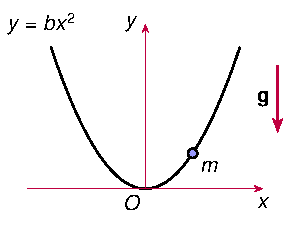
\includegraphics[width=0.8\textwidth]{Figures/Parabol_motion.pdf}
        \vspace{-6mm}
        \caption{Một hạt chuyển động trên bề mặt parabol dưới tác dụng của trọng lực.}
    \end{figure}

\column{0.5\textwidth}
    \begin{itemize}
        \item\textbf{Liên kết phi Holonomic}
    \end{itemize}
    \begin{equation}
        f \left( \mathbf{q}, \dot{\mathbf{q}}, t \right) = 0.
    \end{equation}
    \vspace{-9mm}
    \begin{figure}
        \centering
        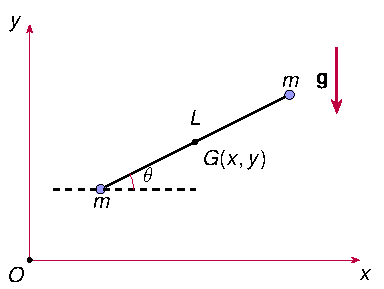
\includegraphics[width=0.8\textwidth]{Figures/NonHolonomic_example.pdf}
        \vspace{-2mm}
        \caption{Một thanh chuyển động dưới tác dụng của trọng trường.}
    \end{figure}
\end{columns}
\end{frame}

\begin{frame}{Bậc tự do}
    \vspace{-4mm}
\begin{columns}
\column{0.6\textwidth}
    \begin{itemize}
        \item \textbf{Số bậc tự do} \\
        \(= \) số tọa độ suy rộng \( - \) số liên kết.
    \end{itemize}
    \begin{itemize}
        \item Ví dụ: con lắc kép.
    \end{itemize}
    \textbf{Cách 1:} Sử dụng 4 tọa độ suy rộng \(\left( x_A, y_A, x_B, y_B \right)\).

    Các liên kết:
    \vspace{-2mm}
    \begin{align}
        f_1 &= x_A^2 + y_A^2 - l_1^2 = 0, \\
        f_2 &= \left( x_B - x_A \right)^2 + \left( y_B - y_A \right)^2 - l_2^2 = 0.
    \end{align}

    \vspace{-2mm}
    Suy ra số bậc tự do: \(4 - 2 = 2\)

    \textbf{Cách 2:} Sử dụng 2 tọa độ suy rộng \(\left( q_1, q_2 \right)\), không có liên kết giữa \(q_1\) và \(q_2\).

    Suy ra số bậc tự do: \(2 - 0 = 2\)

    
\column{0.4\textwidth}
    \begin{figure}
        \centering
        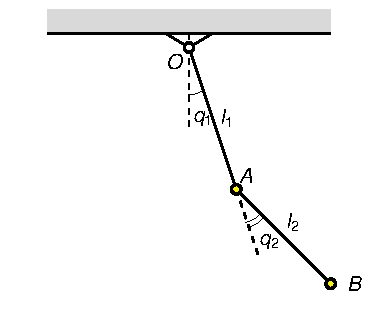
\includegraphics[width=0.9\textwidth]{Figures/Double_pendulum.pdf}
        \caption{Con lắc kép.}
    \end{figure}
\end{columns}
\end{frame}

\subsection{Jacobian và liên hệ vận tốc giữa các hệ tọa độ}

\begin{frame}{Robot Scara 4 bậc tự do}
    \begin{columns}
        \column{0.5\textwidth}
        \begin{itemize}
            \item Robot Scara có 4 bậc tự do biểu diễn qua các tọa độ: \( q = [q_1, q_2, q_3, q_4]^T \).
            \item 3 khớp quay: \(q_1\), \(q_2\), \(q_4\).
            \item 1 khớp tịnh tiến: \(q_3\).
        \end{itemize}
        \begin{figure}
            \centering
            \includegraphics[width=0.8\linewidth]{Figures/Scara_xOz.png}
            \caption{Mặt cắt phương xOz của Robot Scara.}
            \label{fig:Scara_xOz}
        \end{figure}
        \column{0.5\textwidth}
        \begin{figure}
            \centering
            \includegraphics[width=0.8\linewidth]{Figures/Scara_xOy.png}
            \caption{Mặt cắt phương xOy của Robot Scara.}
            \label{fig:Scara_xOy}
        \end{figure}
    \end{columns}
\end{frame}

\begin{frame}{Ma trận Jacobian và liên hệ vận tốc giữa các tọa độ}
    \begin{columns}
        \column{0.5\textwidth}
            \begin{itemize}
                \item Cho hai hệ tọa độ: \( q = \left[ q_1, q_2, q_3 \right]^T\) và \( P = \left[ x, y, z \right]^T\).
                \item Dựa vào phép đạo hàm toàn phần
            \end{itemize}
            \begin{align}
                \dot{x} &= \dfrac{\partial x}{\partial q_1} \dot{q}_1 + \dfrac{\partial x}{\partial q_2} \dot{q}_2 + \dfrac{\partial x}{\partial q_3} \dot{q}_3, \\
                \dot{y} &= \dfrac{\partial y}{\partial q_1} \dot{q}_1 + \dfrac{\partial y}{\partial q_2} \dot{q}_2 + \dfrac{\partial y}{\partial q_3} \dot{q}_3, \\
                \dot{x} &= \dfrac{\partial x}{\partial q_1} \dot{q}_1 + \dfrac{\partial z}{\partial q_2} \dot{z}_2 + \dfrac{\partial z}{\partial q_3} \dot{q}_3.
            \end{align}
        \column{0.5\textwidth}
            \begin{itemize}
                \item Ma trận Jacobian
            \end{itemize}
            \begin{equation}
                J = \left[ \begin{array}{ccc}
                    \dfrac{\partial x}{\partial q_1} & \dfrac{\partial x}{\partial q_2} & \dfrac{\partial x}{\partial q_3} \\
                    \dfrac{\partial y}{\partial q_1} & \dfrac{\partial y}{\partial q_2} & \dfrac{\partial y}{\partial q_3} \\
                    \dfrac{\partial x}{\partial q_1} & \dfrac{\partial z}{\partial q_2} & \dfrac{\partial z}{\partial q_3}
                \end{array} \right].
            \end{equation}
            \begin{itemize}
                \item Ứng dụng: \(\dot{P} = J \dot{q}\).
            \end{itemize}
    \end{columns}
\end{frame}

\begin{frame}{Ma trận Jacobian và liên hệ vận tốc giữa các tọa độ}
    \begin{itemize}
        \item Ứng dụng cho Robot Scara.
    \end{itemize}
            \begin{align}
                \dot{x} &= \left[ -a_1 \sin \left( q_1 \right) - a_2 \sin \left( q_1 + q_2 \right) \right] \dot{q}_1 - a_2 \sin \left( q_1 + q_2 \right) \dot{q}_2, \\
                \dot{y} &= \left[ a_1 \cos \left( q_1 \right) + a_2 \cos \left( q_1 + q_2 \right) \right] \dot{q}_1 - a_2 \cos \left( q_1 + q_2 \right) \dot{q}_2, \\
                \dot{z} &= -\dot{q}_3.
            \end{align}
    \begin{itemize}
        \item Tính độ lớn vận tốc
    \end{itemize}
    \begin{equation}
        v^2 = \dot{x}^2 + \dot{y}^2 + \dot{z}^2
        = \left[ \begin{array}{ccc}
            \dot{x} & \dot{y} & \dot{z}
        \end{array} \right]
        \left[ \begin{array}{c}
            \dot{x} \\
            \dot{y} \\
            \dot{z}
        \end{array} \right]
        = \dot{P}^T \dot{P}
        = \dot{q}^T \left( J^T J \right) \dot{q}.
    \end{equation}
\end{frame}

\section{Động lực học robot}

\subsection{Động năng và ma trận quán tính}

\input{Slides/Mass_matrix}

\subsection{Phương trình động lực học đầy đủ và ma trận Christoffel}

\input{Slides/Lagrangian}

\subsection{Mô phỏng chuyển động bằng phương pháp số}

\section{Phương pháp số trong mô phỏng}\label{sec_2}

Phần này có mục đích giới thiệu một số phương pháp số thường được sử dụng trong mô phỏng vật lý (phương pháp sai phân hữu hạn và phương pháp phần tử hữu hạn). Mục đích của các phương pháp số là xấp xỉ nghiệm của các bài toán điều kiện biên mà trong đó việc giải trực tiếp phương trình vi phân là không thể. Một bài toán điều kiện biên thường được biểu diễn bằng một phương trình đạo hàm riêng và các điều kiện biên đi kèm. Phương trình Poisson 1D trong \cref{eq_PTpoisson_tq} là một ví dụ của bài toán điều kiện biên. Bài toán này có thể giải một cách trực tiếp nếu hàm $f(x)$ là một hàm đơn giản và có thể tích phân. Tuy nhiên trong thực tế, một hàm như vậy không tồn tại nhiều. Vì vậy các phương pháp số đã được phát triển để giải quyết vấn đề này.

\begin{equation}\label{eq_PTpoisson_tq}
    \begin{aligned}
        -\frac{\partial^2u}{\partial x^2} &= f(x) \quad x \in \left(0, L\right) \\
        u\left(0\right) &= u_0 \quad \left(\hbox{điều kiện biên Dirichlet}\right) \\
        \frac{\partial u}{\partial x} \left(L\right) &= u'_L \quad \left(\hbox{điều kiện biên Neumann}\right) \\
    \end{aligned}
\end{equation}

Trong phần còn lại, để đơn giản việc trình bày, chúng ta sẽ chọn $f(x) = x$, $u_0 = 2$ và $u'_L = 1$. Tập xác định của phương trình là $(0, 1)$ (\cref{eq_PTpoisson}). Điều này không làm mất đi tính tổng quát của các phương pháp số, bởi vì việc áp dụng các phương pháp là như nhau cho bất kỳ bài toán điều kiện biên nào.

\begin{equation}\label{eq_PTpoisson}
    \begin{aligned}
        -\frac{\partial^2u}{\partial x^2} &= x \quad x \in \left(0, 1\right) \\
        u\left(0\right) &= 2 \quad \left(\hbox{điều kiện biên Dirichlet}\right) \\
        \frac{\partial u}{\partial x} \left(1\right) &= 1 \quad \left(\hbox{điều kiện biên Neumann}\right) \\
    \end{aligned}
\end{equation}

Với phương trình \cref{eq_PTpoisson}, chúng ta có thể xác định được nghiệm chính xác của nó:

\begin{equation}\label{eq_sol}
    u\left(x\right) = \frac{-x^3 + 9x + 12}{6}
\end{equation}

Các phương pháp số sẽ được áp dụng để giải \cref{eq_PTpoisson} và so sánh với nghiệm chính xác của nó (\cref{eq_sol}).

\subsection{Phương trình vi phân}

Trước khi tìm hiểu các phương pháp số chúng ta cần tìm hiểu một số các biểu diễn các phương trình vi phân, bởi vì với mỗi phương pháp được trình bày sẽ tiếp cận một dạng khác nhau của phương trình.

\subsubsection{Phương trình dạng mạnh}

Phương trình vi phân dạng mạnh là các phương trình mô tả các hiện tương vật lý mà trong đó nghiệm của phương trình thỏa mãn với mọi điểm trong miền xác định. Phương trình Poisson trong \cref{eq_PTpoisson} là một phương trình dạng mạnh. 

\subsubsection{Phương trình dạng yếu}

Phương trình dạng yếu được biểu diễn dưới dạng tích phân của tích phương trình dạng mạnh với một hàm thử trên miền xác định. Ý tưởng là xấp xỉ nghiệm của phương trình dạng mạnh bằng một hàm đơn giản hơn mà việc xác định nó không yêu cầu giải trực tiếp bài toán điều kiện biên. Một trong nhưng phương pháp để biến đổi phương trình dạng mạnh về phương trình dạng yếu đó là phương pháp Ritz-Galerkin.

Chúng ta sẽ bắt đầu bằng việc xấp xỉ nghiệm $u$ của phương trình \cref{eq_PTpoisson} bằng một nghiệm $u^h$. Nghiệm xấp xỉ này sẽ thỏa mãn điều kiện Dirichlet (ie. $u^h(0) = 2$). Vì đây là nghiệm xấp xỉ nên hiển nhiên rằng nghiệm này sẽ không thỏa mãn phương trình vi phân cũng như điều kiện biên Neumann. Vì vậy chúng ta có:

\begin{equation}\label{eq_RR}
    \begin{aligned}
        R_{\Omega} &= -\frac{\partial^2 u^h}{\partial x^2} - x \neq 0 \quad x \in \left(0, 1\right) \\
        R_{\partial\Omega} &= \frac{\partial u^h}{\partial x} \left(1\right) - 1 \neq 0 \\
    \end{aligned}
\end{equation}

Ý tưởng của phương pháp Ritz-Galerkin là nhân các phương trình trong \cref{eq_RR} với một hàm thử $v$ và tích phân trên toàn miền bài toán để tìm nghiệm. Hàm thử này phải thỏa mãn điều kiện Dirichlet \textbf{đồng nhất} $v(0) = 0$. Vì vậy chúng ta có:

\begin{equation}\label{eq_Ritz}
    \begin{aligned}
        &\int\limits_0^1 v R_{\Omega}dx + v(1)R_{\partial\Omega} = 0 \\
        \Rightarrow &\int\limits_0^1 v \left(-\frac{\partial^2 u^h}{\partial x^2} - x\right)dx + v(1)\left(\frac{\partial u^h}{\partial x} \left(1\right) - 1\right) =0
    \end{aligned}
\end{equation}

Sử dụng tích phân từng phần để biến đổi, chúng ta có:

\begin{equation}\label{eq_weakform}
    \int\limits_0^1 \frac{\partial u^h}{\partial x} \frac{\partial v}{\partial x}dx - v(1) - \int\limits_0^1 v x dx =0
\end{equation}

Phương trình \cref{eq_weakform} được gọi là phương trình dạng yếu. Theo nguyên lý Bubnov-Galerkin, hàm thử $v$ sẽ được chọn sao cho nó có cùng hàm nội suy với nghiệm xấp xỉ $u^h$. Việc xác định các hàm nội suy sẽ được trình bày trong phần phương pháp phần tử hữu hạn.

\subsection{Phương pháp số}

\subsubsection{Phương pháp sai phân hữu hạn}

Phương pháp sai phân hữu hạn là phương pháp xấp xỉ nghiệm trực tiếp từ phương trình dạng mạnh. Ý tưởng của phương pháp này là sử dụng chuỗi Taylor để xấp xỉ các đạo hàm và thay vào phương trình vi phân.

\begin{equation}\label{eq_taylor}
    \begin{aligned}
        f(x+h) &=f(x)+f^{\prime}(x) h+\frac{f^{\prime \prime}(x)}{2!} h^2+\frac{f^{\prime \prime \prime}(x)}{3!} h^3+\frac{f^{(4)}\left(\xi_1\right)}{4!} h^4 + \dots\\
        f(x-h) &=f(x)-f^{\prime}(x) h+\frac{f^{\prime \prime}(x)}{2!} h^2-\frac{f^{\prime \prime \prime}(x)}{3!} h^3+\frac{f^{(4)}\left(\xi_2\right)}{4!} h^4 + \dots
\end{aligned}
\end{equation}

Từ đây, chúng ta có các cách để xấp xỉ đạo hàm bậc nhất như sau:

\begin{equation}\label{eq_bac1}
    \begin{aligned}
        f^{\prime}(x) &\approx \frac{f(x+h) - f(x)}{h} \quad \hbox{sai phân tiến} \\
        f^{\prime}(x) &\approx \frac{f(x) - f(x-h)}{h} \quad \hbox{sai phân lùi} \\
        f^{\prime}(x) &\approx \frac{f(x+h) - f(x-h)}{2h} \quad \hbox{sai phân trung tâm} \\
    \end{aligned}
\end{equation}

\textcolor{red}{Chứng minh rằng sai số của sai phân trung tâm thì bé hơn sai phân tiến và sai phân lùi}. Tương tự, ta có thể xấp xỉ đạo hàm bậc 2:

\begin{equation}\label{eq_bac2}
    f^{\prime \prime}(x) \approx \frac{f(x+h) -2f(x) + f(x-h)}{h^2}
\end{equation}

Áp dụng cho ví dụ của chúng ta. Giả sử ta chia miền $x \in (0, 1)$ thành $N=3$ điểm lưới đều với khoảng cách giữa các điểm là $h = \frac{1}{N-1}$. Ta có thể xấp xỉ đạo hàm bậc 2 của hàm $u$ tại điểm $x_2$ như sau:

\begin{equation}
    - \frac{u_1 - 2u_2 +u_3}{h^2} = x_2
\end{equation}

Điều kiện biên Neumann được xấp xỉ bằng cách sử dụng sai phân lùi:

\begin{equation}
    \frac{u_3 -u_2}{h} = 1
\end{equation}

Kết hợp 2 PT trên và điều kiện biên Dirichlet, ta có hệ phương trình:

\begin{equation}
    \begin{bmatrix}
        1 & 0 & 0 \\ 1/h^2 & -2/h^2 & 1/h^2 \\ 0 & -1/h & 1/h 
    \end{bmatrix}\begin{bmatrix}
        u_1 \\ u_2 \\ u_3 
    \end{bmatrix} = \begin{bmatrix}
        2 \\ -x_2 \\ 1
    \end{bmatrix}
\end{equation}

Giải phương trình tuyến tính trên ta sẽ thu được giá trị tại các nút. Kết quả của phương pháp này phụ thuộc vào độ mịn của lưới chia. Nếu lưới chia quá thô thì kết quả sẽ không chính xác. Tuy nhiên nếu lưới chia quá mịn thì sẽ dẫn đến việc tính toán tốn thời gian và tài nguyên máy tính. Số lượng nút chia lưới sẽ ảnh hưởng đến độ chính xác của phương pháp này. Với 3 nút thì kết quả thu được có sai số khá lớn so với nghiệm chính xác. Tuy nhiên nếu tăng số lượng nút lên thì kết quả sẽ gần với nghiệm chính xác hơn (xem \cref{fig_SPHHresults}).

\begin{figure}[htbp]
    \centering
    \begin{subfigure}[b]{0.3\linewidth}
        \centering
        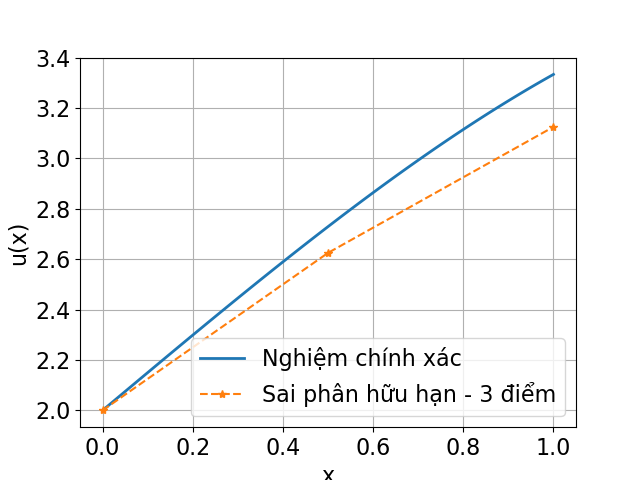
\includegraphics[width=\linewidth]{Tuan6/figure/SPHH_3p.png}
        \caption{3 nút}
        \label{fig:SPHH_3p}
    \end{subfigure}\hfill
    \begin{subfigure}[b]{0.3\linewidth}
        \centering
        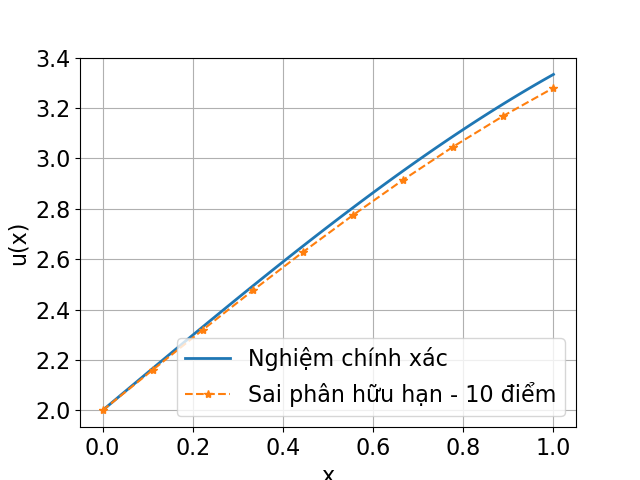
\includegraphics[width=\linewidth]{Tuan6/figure/SPHH_10p.png}
        \caption{10 nút}
        \label{fig:SPHH_10p}
    \end{subfigure}\hfill
    \begin{subfigure}[b]{0.3\linewidth}
        \centering
        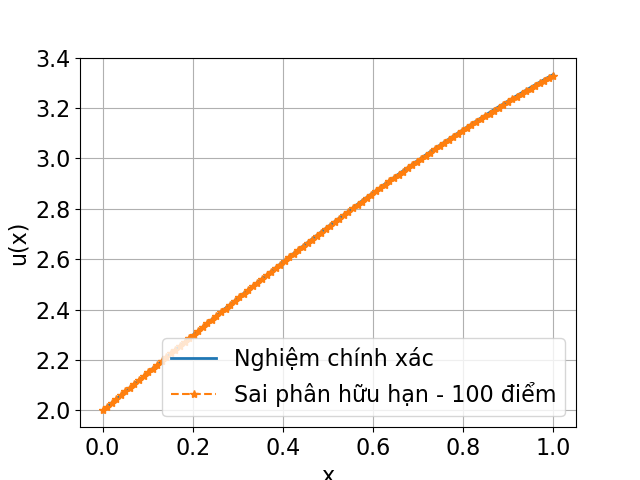
\includegraphics[width=\linewidth]{Tuan6/figure/SPHH_100p.png}
        \caption{100 nút}
        \label{fig:SPHH_100p}
    \end{subfigure}
    \caption{Nghiệm của PT Poisson bằng phương pháp sai phân hữu hạn với (a) 3 nút, (b) 10 nút, (c) 100 nút.}
    \label{fig_SPHHresults}
\end{figure}


\subsubsection{Phương pháp phần tử hữu hạn}

Ý tưởng của phương pháp này là chia miền xác định thành các miền con $\Omega_e$ không giao nhau gọi là các phần tử (chia lưới). Các phần tử liên kết với nhau tại các nút đặt tại các đỉnh của phần tử. Đối với miền 1D thì phần tử là các đoạn thẳng có các nút ở 2 đầu. Miền 2D thì phần tử là các đa giác (thường là tam giác hoặc tứ giác với nút đặt tại các đỉnh). 

Xét bài toán 1D, miền xác định được chia thành m miền con, số nút tương ứng là $n = m+1$,mỗi nút có tọa độ $x_i$, mỗi phần tử giới hạn bởi $\Omega_e = [x_i, x_{i+1}]$. Mỗi nút liên kết với 1 hàm dạng (hàm nội suy) $N_i(x)$. Hàm dạng thường là các hàm đa thức thỏa mãn tính chất $N_i(x_i) = 1$ và $N_i(x_j) = 0$ với $j \neq i$.

Nghiệm xấp xỉ theo phương pháp phần tử hữu hạn lúc này sẽ được biểu diễn bởi 

\begin{equation}\label{eq_interpolation}
    u^h(x) = \sum\limits_{i=1}^n N_i(x) u_i = \underbrace{\begin{bmatrix}
        N_1(x) \dots N_n(x)
    \end{bmatrix}}_{{\bf N}(x)} \underbrace{\begin{bmatrix}
        u_1 \\ \vdots \\ u_n 
    \end{bmatrix}}_{\bf u}
\end{equation}

Vector ${\bf u}$ chứa các phần tử là giá trị của $u^h(x)$ tại các nút và được gọi là bậc tự do của bài toán. Chia lưới càng mịn thì sẽ dẫn đến số lượng bậc tự do sẽ tăng lên càng nhiều nhưng kết quả sẽ càng chính xác.

Theo nguyên lý Bubnov-Galerkin, hàm thử $v$ sẽ được chọn sao cho nó có cùng hàm nội suy với nghiệm xấp xỉ $u^h$. Vì vậy ta có:

\begin{equation}\label{eq_interpolation_test}
    v(x) = \sum\limits_{i=1}^n N_i(x) v_i = {{\bf N}(x)}{\bf v}
\end{equation}

Thay các xấp xỉ này vào \cref{eq_weakform}, ta có:

\begin{equation}
    {\bf v}^T\left(\int\limits_0^1\left(\frac{\partial{\bf N}}{\partial x}\right)^T\frac{\partial{\bf N}}{\partial x} dx\right){\bf u} - {\bf v}^T[{\bf N}(1)]^T - {\bf v}^T\int\limits_0^1 [{\bf N}(x)]^Tx dx = 0
\end{equation}

Rút gọn PT trên, ta có:

\begin{equation}\label{eq_matrixform}
    \underbrace{\left(\int\limits_0^1\left(\frac{\partial{\bf N}}{\partial x}\right)^T\frac{\partial{\bf N}}{\partial x} dx\right)}_{\bf K}{\bf u} = \underbrace{[{\bf N}(1)]^T + \int\limits_0^1 [{\bf N}(x)]^Tx dx}_{\bf F} 
\end{equation}

Giải PT \cref{eq_matrixform}, chúng ta sẽ tìm được giá trị của vector bac tu do. ${\bf u} = {\bf K}^{-1}{\bf F}$.

Việc còn lại bây giờ là xác định các hàm dạng $N_i(x)$ và ma trận ${\bf K}$, ${\bf F}$. Các hàm dạng này sẽ được xác định dựa trên hình dạng của phần tử. Đối với miền 1D, các phần tử là các đoạn thẳng nối các nút với nhau. Hàm dạng sẽ là các hàm nội suy tuyến tính. Hàm dạng tuyến tính 1D được biểu diễn như sau (\cref{eq_shape1D,fig_shape_func}):

\begin{equation}\label{eq_shape1D}
    \begin{aligned}
        N_1(x) &= \frac{1}{x_2-x_1}\left(x_2-x\right) \\
        N_2(x) &= \frac{1}{x_2-x_1}\left(x-x_1\right) \\
    \end{aligned}
\end{equation}

\begin{figure}[htbp]
    \centering
    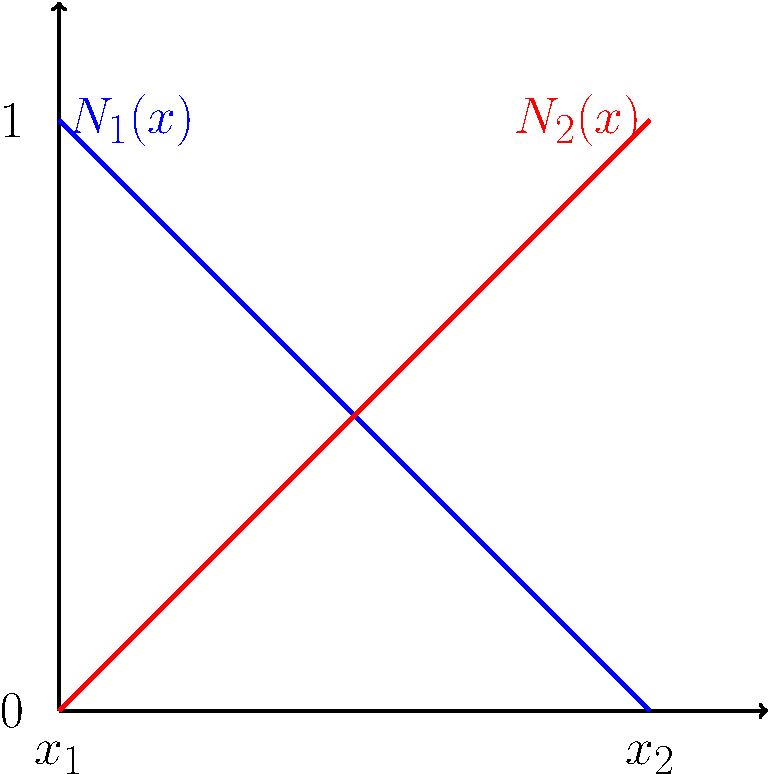
\includegraphics[width=0.3\linewidth]{Tuan6/figure/shape_func.pdf}
    \caption{Ham noi suy 1D}
    \label{fig_shape_func}
\end{figure}

Chúng ta có thể thấy rằng các hàm dạng là như nhau đối với các phần tử có hình dạng giống nhau. Đây là điểm đặc biệt của phương pháp phần tử hữu hạn. Giả sử miền tích phân được chia thành 100 phần tử với 101 nút thì chúng ta không cần phải tích phân để tìm từng phần tử trong ma trận ${\bf K}$, mà thay vào đó chúng ta xác định ma trận ${\bf K}_e$ của từng phần tử và \textbf{lắp ráp} chúng vào ma trận ${\bf K}$. Ví dụ sau đây sẽ minh họa cách lắp ráp ma trận ${\bf K}$ từ ma trận ${\bf K}_e$ của từng phần tử.

Quay lại với phương trình Poisson 1D, chúng ta sẽ xác định ma trận ${\bf K}_e$ của một phần tử giới hạn bởi $[x_1, x_2]$. Đặt $L_e = x_2 -x_1$, ta có:

\begin{equation}\label{eq_Ke}
    \begin{aligned}
        {\bf K}_e &= \int\limits_{x_1}^{x_2}\left(\frac{\partial{\bf N}}{\partial x}\right)^T\frac{\partial{\bf N}}{\partial x} dx \\
        & =\int\limits_{x_1}^{x_2}\begin{bmatrix}
            \frac{\partial N_1}{\partial x} \\ \frac{\partial N_2}{\partial x}
        \end{bmatrix}\begin{bmatrix}
            \frac{\partial N_1}{\partial x} &\frac{\partial N_2}{\partial x}
        \end{bmatrix}dx = \int\limits_{x_1}^{x_2}\begin{bmatrix}
            \frac{-1}{L_e} \\ \frac{1}{L_e}
        \end{bmatrix}\begin{bmatrix}
            \frac{-1}{L_e}& \frac{1}{L_e}
        \end{bmatrix}dx \\
        &= \int\limits_{x_1}^{x_2}\begin{bmatrix}
            \frac{1}{L_e^2} & \frac{-1}{L_e^2} \\
            \frac{-1}{L_e^2} & \frac{1}{L_e^2}
        \end{bmatrix}dx = \begin{bmatrix}
            \frac{1}{L_e} & \frac{-1}{L_e} \\
            \frac{-1}{L_e} & \frac{1}{L_e}
        \end{bmatrix} = \begin{bmatrix}
            K_{11} & K_{12} \\
            K_{21} & K_{22}
        \end{bmatrix}
    \end{aligned}
\end{equation}

Số hạng $ \int\limits_0^1 [{\bf N}(x)]^Tx dx$ cũng được tính bằng cách tương tự:

\begin{equation}
    \begin{aligned}
        \int\limits_{x_1}^{x_2} [{\bf N}(x)]^Tx dx &= \int\limits_{x_1}^{x_2} \begin{bmatrix}
            N_1 \\ N_2
        \end{bmatrix}x dx \\
        & = \int\limits_{x_1}^{x_2}\begin{bmatrix}
            \frac{x_2-x}{L_e} \\ \frac{x-x_1}{L_e}
        \end{bmatrix}x dx = \begin{bmatrix}
            \frac{x_2^3-3x_2x_1^2+2x_1^3}{6L_e} \\ \frac{2x_2^3-3x_1x_2^2+x_1^3}{6L_e}
        \end{bmatrix} = \begin{bmatrix}
            F_1 \\ F_2
        \end{bmatrix}
    \end{aligned}
\end{equation}

Chúng ta đã xác định được ma trận ${\bf K}_e$ và vector ${\bf F}_e$ cho một phần tử. Bây giờ chúng ta sẽ lắp ráp chúng để có ma trận toàn cục ${\bf K}$ và vector ${\bf F}$.

Giả sử miền tích phân được chia thành 2 phần tử $e1$ và $e2$ với các nút lần lượt là $x_1 = 0$, $x_2 = 0.5$, $x_3 = 1$. Vector bậc tự do của chúng ta sẽ là ${\bf u} = [u_1 \; u_2 \; u_3]^T$. Trong đó nút 2 sẽ là điểm kết nối giữa 2 phần tử, vì vậy $u_2 = u_2^{e1} + u_2^{e2}$. Ta có:

\begin{equation}
    {\bf K}_{e1}{\bf u}_{e1} = \begin{bmatrix}
        K_{11}^{e1} & K_{12}^{e1} \\
        K_{21}^{e1} & K_{22}^{e1}
    \end{bmatrix}\begin{bmatrix}
        u_1 \\ u_2^{e1}
    \end{bmatrix} \quad \hbox{va} \quad {\bf K}_{e2}{\bf u}_{e2} = \begin{bmatrix}
        K_{22}^{e2} & K_{23}^{e2} \\
        K_{32}^{e2} & K_{33}^{e2}
    \end{bmatrix}\begin{bmatrix}
        u_2^{e2} \\ u_3
    \end{bmatrix}
\end{equation}

Kết hợp 2 PT trên với lưu ý rằng $u_2 = u_2^{e1} + u_2^{e2}$, ta có:

\begin{equation}
    {\bf K}{\bf u} = \begin{bmatrix}
        K_{11}^{e1} & K_{12}^{e1} & 0\\
        K_{21}^{e1} & K_{22}^{e1}+K_{22}^{e2} & K_{23}^{e2} \\
        0 & K_{32}^{e2} & K_{33}^{e2}
    \end{bmatrix}\begin{bmatrix}
        u_1 \\ u_2 \\ u_3
    \end{bmatrix}
\end{equation}

làm tương tự với tích phân $ \int\limits_0^1 [{\bf N}(x)]^Tx dx$, ta có:

\begin{equation}
    \int\limits_0^1 [{\bf N}(x)]^Tx dx = \begin{bmatrix}
        F_1^{e1} \\ F_2^{e1}+F_2^{e2} \\ F_3^{e2}
    \end{bmatrix}
\end{equation}

Thay vào phương trình \cref{eq_matrixform}, ta có:

\begin{equation}
    \begin{bmatrix}
        K_{11}^{e1} & K_{12}^{e1} & 0\\
        K_{21}^{e1} & K_{22}^{e1}+K_{22}^{e2} & K_{23}^{e2} \\
        0 & K_{32}^{e2} & K_{33}^{e2}
    \end{bmatrix}\begin{bmatrix}
        u_1 \\ u_2 \\ u_3
    \end{bmatrix} = \begin{bmatrix}
        0 \\ 0 \\ 1
    \end{bmatrix} + \begin{bmatrix}
        F_1^{e1} \\ F_2^{e1}+F_2^{e2} \\ F_3^{e2}
    \end{bmatrix}
\end{equation}

Thay số cụ thể vào, ta có:

\begin{equation}
    \begin{bmatrix}
        2 & -2 & 0\\
        -2 & 2+2 & -2 \\
        0 & -2 & 2
    \end{bmatrix}\begin{bmatrix}
        u_1 \\ u_2 \\ u_3
    \end{bmatrix} = \begin{bmatrix}
        1/24 \\ 1/12 + 1/6 \\ 5/24 + 1
    \end{bmatrix}
\end{equation}

Phương trình tuyến tính trên không thể giải được vì định thức của ma trận ${\bf K}$ là bằng 0. Điều này xảy ra do điều kiện biên Dirichlet chưa được. Để giải quyết vấn đề này, chúng ta cần loại bỏ một bậc tự do bằng cách áp dụng điều kiện biên Dirichlet ban đầu.

\begin{equation}
    \begin{bmatrix}
        -2 & 4 & -2 \\
        0 & -2 & 2
    \end{bmatrix}\begin{bmatrix}
        2 \\ u_2 \\ u_3
    \end{bmatrix} = \begin{bmatrix}
        1/4 \\ 29/24
    \end{bmatrix} \Leftrightarrow \begin{bmatrix}
        4 & -2 \\
        -2 & 2
    \end{bmatrix}\begin{bmatrix}
        u_2 \\ u_3
    \end{bmatrix} = \begin{bmatrix}
        1/4 \\ 29/24
    \end{bmatrix} - 2\begin{bmatrix}
        -2 \\ 0
    \end{bmatrix}
\end{equation}

Giải phương trình tìm $u_2$ va $u_3$. Chúng ta thu được:

\begin{equation}
    {\bf u} = \begin{bmatrix}
        2 \\ 131/48 \\ 10/3
    \end{bmatrix}
\end{equation}

Dưới đây là các kết quả thu được với số phần tử thay đổi \cref{fig_PTHHresults}:

\begin{figure}[htbp]
    \centering
    \begin{subfigure}[b]{0.3\linewidth}
        \centering
        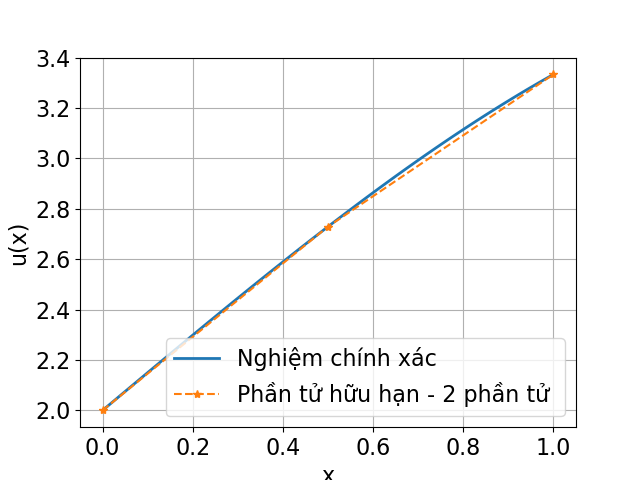
\includegraphics[width=\linewidth]{Tuan6/figure/PTHH_2el.png}
        \caption{}
        \label{fig:PTHH_2el}
    \end{subfigure}\hfill
    \begin{subfigure}[b]{0.3\linewidth}
        \centering
        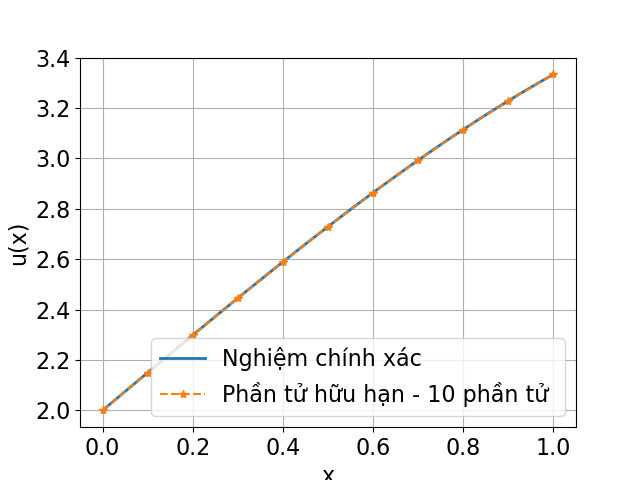
\includegraphics[width=\linewidth]{Tuan6/figure/PTHH_10el.png}
        \caption{}
        \label{fig:PTHH_10el}
    \end{subfigure}\hfill
    \begin{subfigure}[b]{0.3\linewidth}
        \centering
        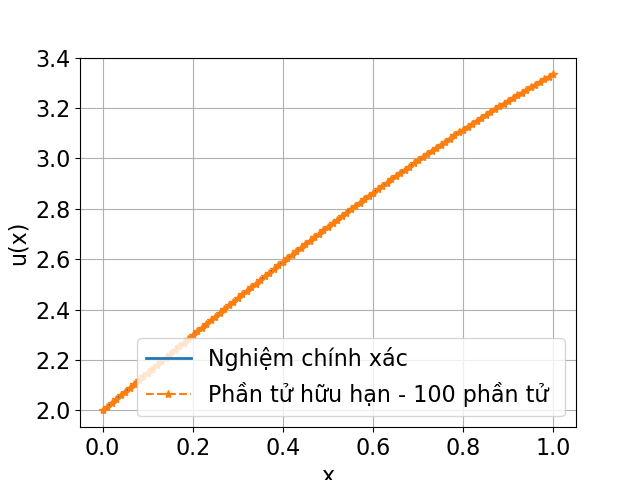
\includegraphics[width=\linewidth]{Tuan6/figure/PTHH_100el.png}
        \caption{}
        \label{fig:PTHH_100el}
    \end{subfigure}
    \caption{Nghiệm của PT Poisson bằng phương pháp phần tử hữu hạn: (a) 2 phần tử, (b) 10 phần tử, (c) 100 phần tử.}
    \label{fig_PTHHresults}
\end{figure}

\textbf{\textcolor{red}{Cau hoi: Đưa ra một số nhận xét về các phương pháp đã trình bày? (ưu điểm, nhược điểm, độ chính xác, xem xét đến khả năng của mỗi phương pháp trong các miền 2D, 3D, etc.)}}

\section{Ma trận còn có thể làm những gì trong cơ học?}

\subsection{Bảng Denavit–Hartenberg}

\input{Slides/Denavit–Hartenberg}

\subsection{Thay thế ma trận Christoffel?}

\input{Slides/Kronecker_product}

\begin{frame}[allowframebreaks]{Tài liệu tham khảo}
    \begin{refsection}
        \nocite{morin2008introduction,calculusjame, 3b1b,griffiths2023introduction}
         \printbibliography
    \end{refsection}
\end{frame}

\end{document}